\documentclass[conf]{new-aiaa}
%\documentclass[journal]{new-aiaa} for journal papers
\usepackage[utf8]{inputenc}

\usepackage{graphicx}
\usepackage{amsmath}
\usepackage[version=4]{mhchem}
\usepackage{siunitx}
\usepackage{longtable,tabularx}
\usepackage{subcaption}
\setlength\LTleft{0pt} 

\begin{document}

\section{Battery Model}

\begin{figure}[hbt!]
\centering
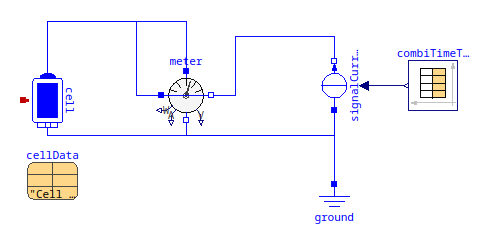
\includegraphics[width=.5\textwidth]{Fig1}
\caption{OpenModelica Model of a 26650 Cell.}
\label{fig:OMModel}
\end{figure}

A model of a 26650 litium-ion battery cell was developed using the standard OpenModelica electrical libraries, pictured in Fig. \ref{fig:OMModel}. The primary components are 1) a single 26650 cell, 2) a "cellData" record containing all the pertinent parameters for the battery model, 3) a variable current load representing the aircraft motor, and 4) voltage, current, and power meters.  The model can easily be scaled from a single cell to a full stack of arbitrary size by specifying the number of cells to be connected in parallel and in series.

Parameterization of the model was done by experiment and review of the literature.  A used K2 LFP26650P was used in all experiments; full manufacturer specifications of the cell are given in Table \ref{tab:spec}.  Because of the degraded state of the battery, the maximum capacity was approximately 85\% of nominal, or 2.21 A-hr.  The two most important parameters in characterization are the SOC-OCV curve and the cell's internal resistance; derivation of these parameters are given below.

\begin{table}[hbt!]
\caption{K2 LFP26650P Manufacturer Specifications}
\label{tab:spec}
\centering
\begin{tabular}{cc}
\hline 
Specification & Value\\
\hline
Diameter, mm & 0.046653\\
Length, mm & 0.031821\\
Cell Capacity at C/5, A-hr & 0.028593\\
Weight, g & 0.023320\\
Operating Temperature, \textdegree C & -20 to 60\\
\hline
\end{tabular}
\end{table}

\subsection{SOC-OCV Curve}
The SOC-OCV curve for a battery maps the open circuit voltage (OCV), the cell's voltage when disconnected from any current load, to the cell's state of charge (SOC), ranging from 0 to 1.  In Chin et. al. \cite{Chin}, the author's develop a comprehensive electro-thermal model of a similar 26650 cell, including the SOC-OCV curve, shown below.

\begin{figure}[hbt!]
\centering
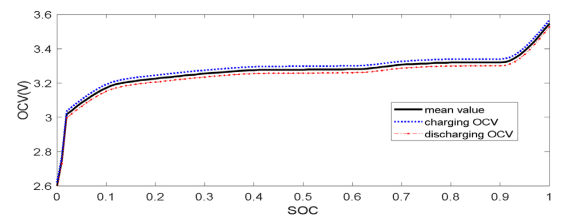
\includegraphics[width=.5\textwidth]{Fig2}
\caption{Average SOC-OCV Curve for a 26650 Cell. \cite{Chin}}
\label{fig:SOCOCV}
\end{figure}

Data from this curve was tabulated and entered as the cell's SOC-OCV curve.  The model then was benchmarked by simulating a full discharge cycle at 5 A and comparing the result to the discharge curve provided by the manufacturer.  A nominal (0.001 $\Omega$) resistance was assumed.  The results showed generally good agreement (Fig. \ref{fig:ManDischarge}), matching to within ~5\% during the constant voltage part of the curve.  The SOC-OCV curve of Chin therefore was deemed adequate.

\begin{figure}[hbt!]
\centering
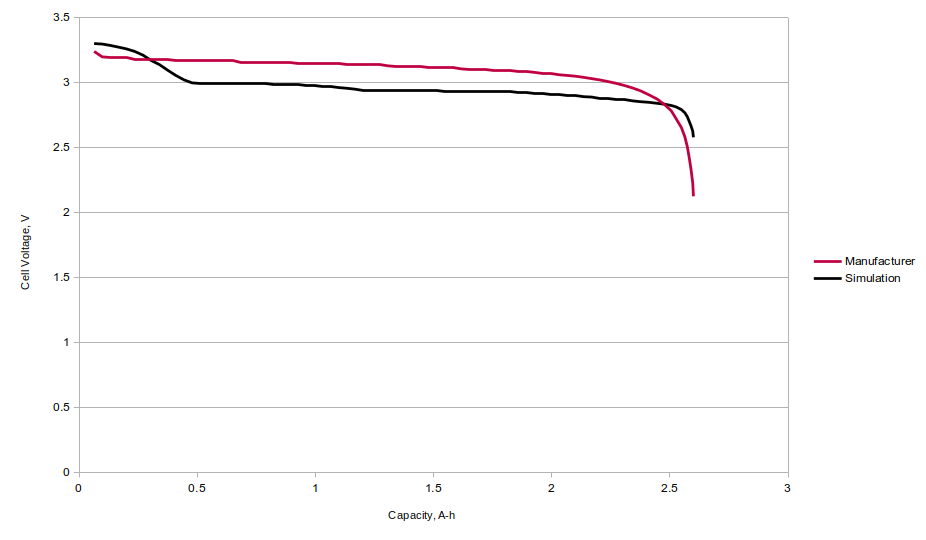
\includegraphics[width=.5\textwidth]{Fig3}
\caption{Manufacturer vs. Simulated Discharge Curve}
\label{fig:ManDischarge}
\end{figure}

\subsection{Internal Resistance}
To estimate a the cell's internal resistance, a series of pulse tests were run at a series of different ambient temperatures (20, 30, 40, and 50 \textdegree C).  In each, the cell was charged at 6 amps and discharged at 3 amps three times.  For each discharge cycle, the cell's voltage drop was measured and the resistance estimated from Ohm's Law.  The calculated resistances from each pulse were then averaged to give an overall value at each temperature.  Full results are given in Table \ref{tab:res}.  To estimate the resistance at an arbitrary ambient, the result for each ambient were fit to an exponential curve, giving:

\begin{table}[hbt!]
\caption{26650 Cell Internal Resistance}
\label{tab:res}
\centering
\begin{tabular}{cc}
\hline 
Ambient Temperature, \textdegree C & Resistance, $\Omega$\\
\hline
20 & 0.046653\\
30 & 0.031821\\
40 & 0.028593\\
50 & 0.023320\\
T$_{amb}$ & 0.069184 exp(-0.022182 T$_{amb}$)\\
\hline
\end{tabular}
\end{table}

\newpage
\subsection{Validation}
To validate the model, a set of discharge tests were conducted measuring the cell's voltage and power, with the measured current being directly input as the current load of the simulated cell.  As in the section on cell resistance, these tests were conducted at 20, 30, 40, and 50 \textdegree C.  A representative example of the results at 50 \textdegree C is shown in Fig. \ref{fig:vala} (cell voltage) and Fig. \ref{fig:valb} (power).  In general, excellent agreement is shown for SOC greater than 0.1 (greater than ~2800 seconds).  The elbow observed below this threshold is likely an artifact of the SOC-OCV curve, and may be ironed out with additional testing.  At the lower ambients, this divergence begins slightly earlier; this is due to the resistance calculations being less reliable at lower temperatures \cite{Chin}.

\begin{figure}[hbt!]
\centering
\begin{subfigure}[t]{0.45\textwidth}
\centering
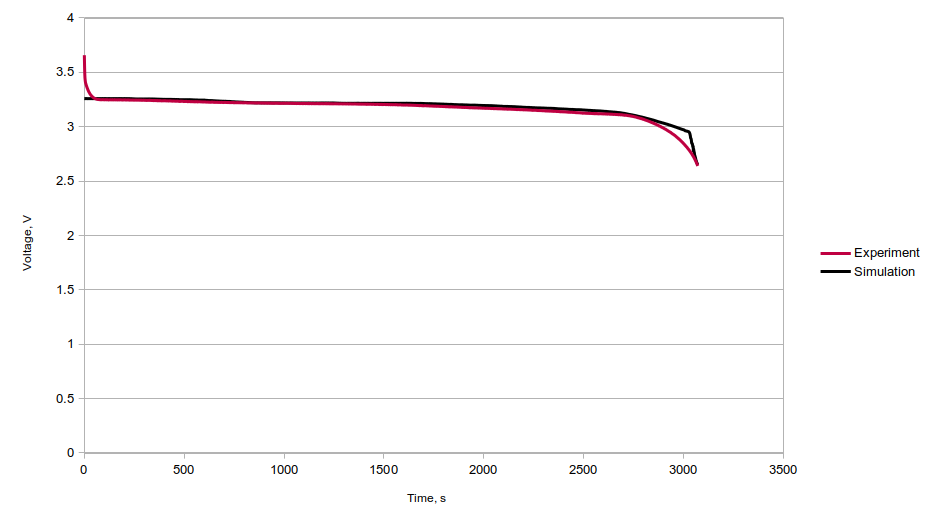
\includegraphics[width=\textwidth]{Fig4a}
\caption{Voltage}
\label{fig:vala}
\end{subfigure}
\begin{subfigure}[t]{0.45\textwidth}
\centering
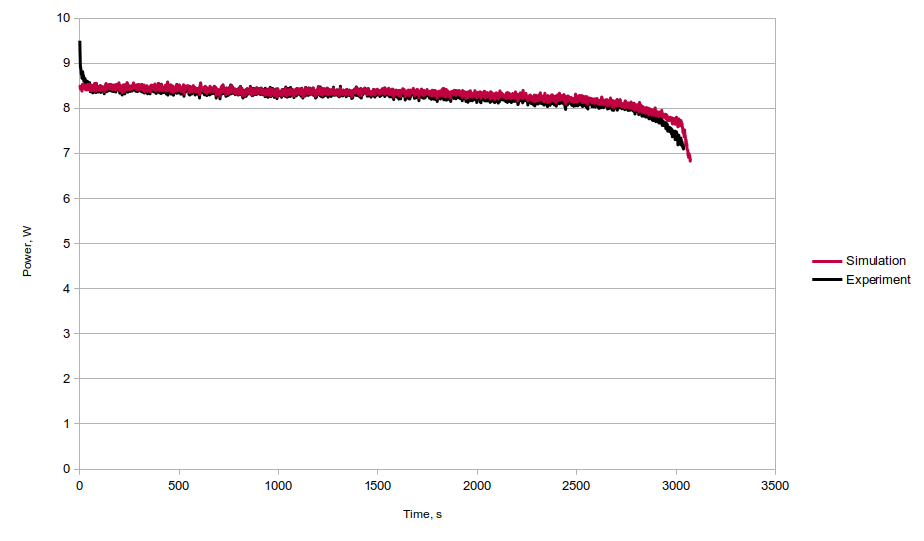
\includegraphics[width=\textwidth]{Fig4b}
\caption{Power}
\label{fig:valb}
\end{subfigure}
\caption{Experimental vs. Simulated Results}
\label{fig:val}
\end{figure}

\bibliography{ref}

\end{document}